%!TEX root = ../thesis.tex
%*******************************************************************************
%****************************** Third Chapter **********************************
%*******************************************************************************
\chapter{Results}

% **************************** Define Graphics Path **************************
\ifpdf
    \graphicspath{{Chapter3/Figs/Raster/}{Chapter3/Figs/PDF/}{Chapter3/Figs/}}
\else
    \graphicspath{{Chapter3/Figs/Vector/}{Chapter3/Figs/}}
\fi

In this chapter we present the performance of the classifiers under the different split schemes outlined earlier. The various features used and their applicability on different splitting conditions is also be evaluated. 

The confusion matrix used will have the form 
\begin{align}
	\begin{bmatrix}
	\text{True Black/ Black Predicted correctly}&\text{False White/ Black  Predicted falsely}\\
	\text{False Black/ White Predicted falsely}&\text{True White/ White  Predicted correctly}
	\end{bmatrix}
\end{align}



The results of the benchmark method we devised in section \ref{sec:splitting} are presented in table \ref{label} for maximum similarit, table \ref{label} for maximum dissimilarity, and table \ref{label} for random splits.


\begin{table}
	\centering
	\begin{tabular}{l c c c}
		\toprule 
		&\multicolumn{2}{c}{Confusion Matrix} &Accuracy\\
		Features used & Predicted Black&Predicted White&\\ 
		
		\midrule
		\multirow{2}{*}{Full OTU }& 	2.64 & 18.36&		\multirow{2}{*}{77.6\%}\\
					&	18.36 &124.64&\\
		\cmidrule{2-3}
		\multirow{2}{*}{Min OTU}  &2.75 & 18.25&		\multirow{2}{*}{76.8\%}\\
		&18.25& 117.75&\\
		\bottomrule
		\hline 
	\end{tabular}
	\caption{Benchmark for Maximum Similarity}
	\label{table:benchmarksim}
\end{table}

\begin{table}
	\centering
	\begin{tabular}{l c c c }
		\toprule 
		&\multicolumn{2}{c}{Confusion Matrix} & Accuracy\\
		Features used & Predicted Black&Predicted White&\\ 
		
		\midrule
		\multirow{2}{*}{Full OTU }&  1.75 &19.25&\multirow{2}{*}{76.7\%}\\
								  &	 18.96&124.04 &\\
		\cmidrule{2-3}
		\multirow{2}{*}{Min OTU}    &1.83&19.17&\multirow{2}{*}{75.8\% }\\
									&18.83&117.17&\\
		\bottomrule
		\hline 
	\end{tabular}
	\caption{Benchmark for Maximum Dissimilarity}
	\label{table:benchmarkdissim}
\end{table}

\begin{table}
\caption{Results from maximising similarity using Logistic Regression}
\centering
\label{table:lrsimilarity}
\begin{tabular}{l c  c}
\hline 
Features used & Mean Score & Variance of Score \\ 
 
\hline
OTU & 98.2\% & 0.04\%   \\
OTU LOW &98.2\% &0.04\%\\
OTU CSS & 96.2\% & 0.13\%   \\
OTU Min CSS & 96.7\% & 0.11\%   \\
OTU CSS LOG & 98.3\% & 0.04\% \\
PCoA Bray-Curtis &96.4\% & 0.13\%   \\
PCoA 99\%      &  96.4\%& 0.13\%\\
PCoA 90\%       & 96.4\% &0.13\%\\
PCoA Bray-Curtis CSS &96.2\% & 0.13\%   \\
PCoA CSS 99\%    &96.2\%&0.14\%\\
PCoA CSS 90\%  &  95.6\% &0.17\%\\
\hline 
\end{tabular}
\end{table}
% RFR similarirtty
\begin{table}
	\caption{Results from maximising similarity using Random Forests Classifier}
	\centering
	\label{table:rfrsimilarity}
	\begin{tabular}{l c  c}
		\hline 
		Features used & Mean Score & Variance of Score \\ 
		
		\hline
		OTU & 90.5\% & 0.14\%   \\
		OTU LOW& 90.4\% &0.11\% \\
		OTU CSS & 94.5\% & 0.07\%   \\
		OTU Min CSS & 94.3\% & 0.08\%   \\
		OTU CSS LOG & 95.1\% & 0.11\% \\
		PCoA Bray-Curtis &87.2\% & 0.19\%   \\
		PCoA Bray Curtis 99\%&        88.5\% &0.29\%\\
		PCoA Bray Curtis 90\% &       89.2\%&0.21\%\\
		PCoA Bray-Curtis CSS 99\% &    89.5\%&0.14\%\\
		PCoA Bray Curtis CSS 90\%   & 92.1\% &0.15\%\\
		PCoA Bray-Curtis CSS &87.2\% & 0.19\%   \\
		
		\hline 
	\end{tabular}
\end{table}


% Logistic Dissimilarity
\begin{table}[h]
\caption{Results from maximising dissimilarity using Logistic Regression}
\centering
\label{table:lrdissimilarity}
\begin{tabular}{l c  c}
\hline 
Features used & Mean Score & Variance of Score \\ 
 
\hline
OTU & 80.7\% & 1.96\%   \\
OTU LOW &82.0\%&1.90\%\\
OTU CSS & 85.7\% & 1.13\%   \\
OTU Min CSS & 84.7\% & 1.40\%   \\
OTU CSS LOG& 91.3\% &1.20\%\\
PCoA Bray-Curtis &88.0\% & 1.00\%   \\
PCoA 99\%&        88.0\%&1.00\%\\
PCoA 90\% &      89.8\%&1.17\%\\
PCoA Bray-Curtis CSS &88.5\% & 1.27\%   \\
PCoA CSS 99\% &   88.\%&1.27\%\\
PCoA CSS 90\%&    85.6\%&1.3\%\\

\hline 
\end{tabular}
\end{table} 

% RFR dissimilarity table
\begin{table}[h]
	\caption{Results from maximising dissimilarity using Random Forest Classifier}
	\centering
	\label{table:rfrdissimilarity}
	\begin{tabular}{l c  c}
		\hline 
		Features used & Mean Score & Variance of Score \\ 
		
		\hline
		OTU & 88.0\% & 2.42\%   \\
		OTU LOW &88.7\%&2.55\%\\
		OTU CSS & 88.0\% & 2.42\%   \\
		OTU Min CSS & 88.5\% & 2.66\%   \\
		OTU CSS LOG & 89.2\%&	2.30\%\\
		PCoA Bray-Curtis &88.0\% & 2.42\%   \\
		PCoA Bray-Curtis 99\% &88.0\% & 2.42\%   \\
		PCoA Bray-Curtis 90\%&88.0\% & 2.42\%   \\
		PCoA Bray-Curtis CSS &88.5\% & 2.42\%   \\
		PCoA Bray-Curtis CSS 99\%&88.0\% & 2.42\%   \\
		PCoA Bray-Curtis CSS 90\%&88.0\% & 2.42\%   \\		
		\hline 
	\end{tabular}
\end{table} 



\begin{figure}
	\centering
	\begin{subfigure}{0.45\textwidth}
		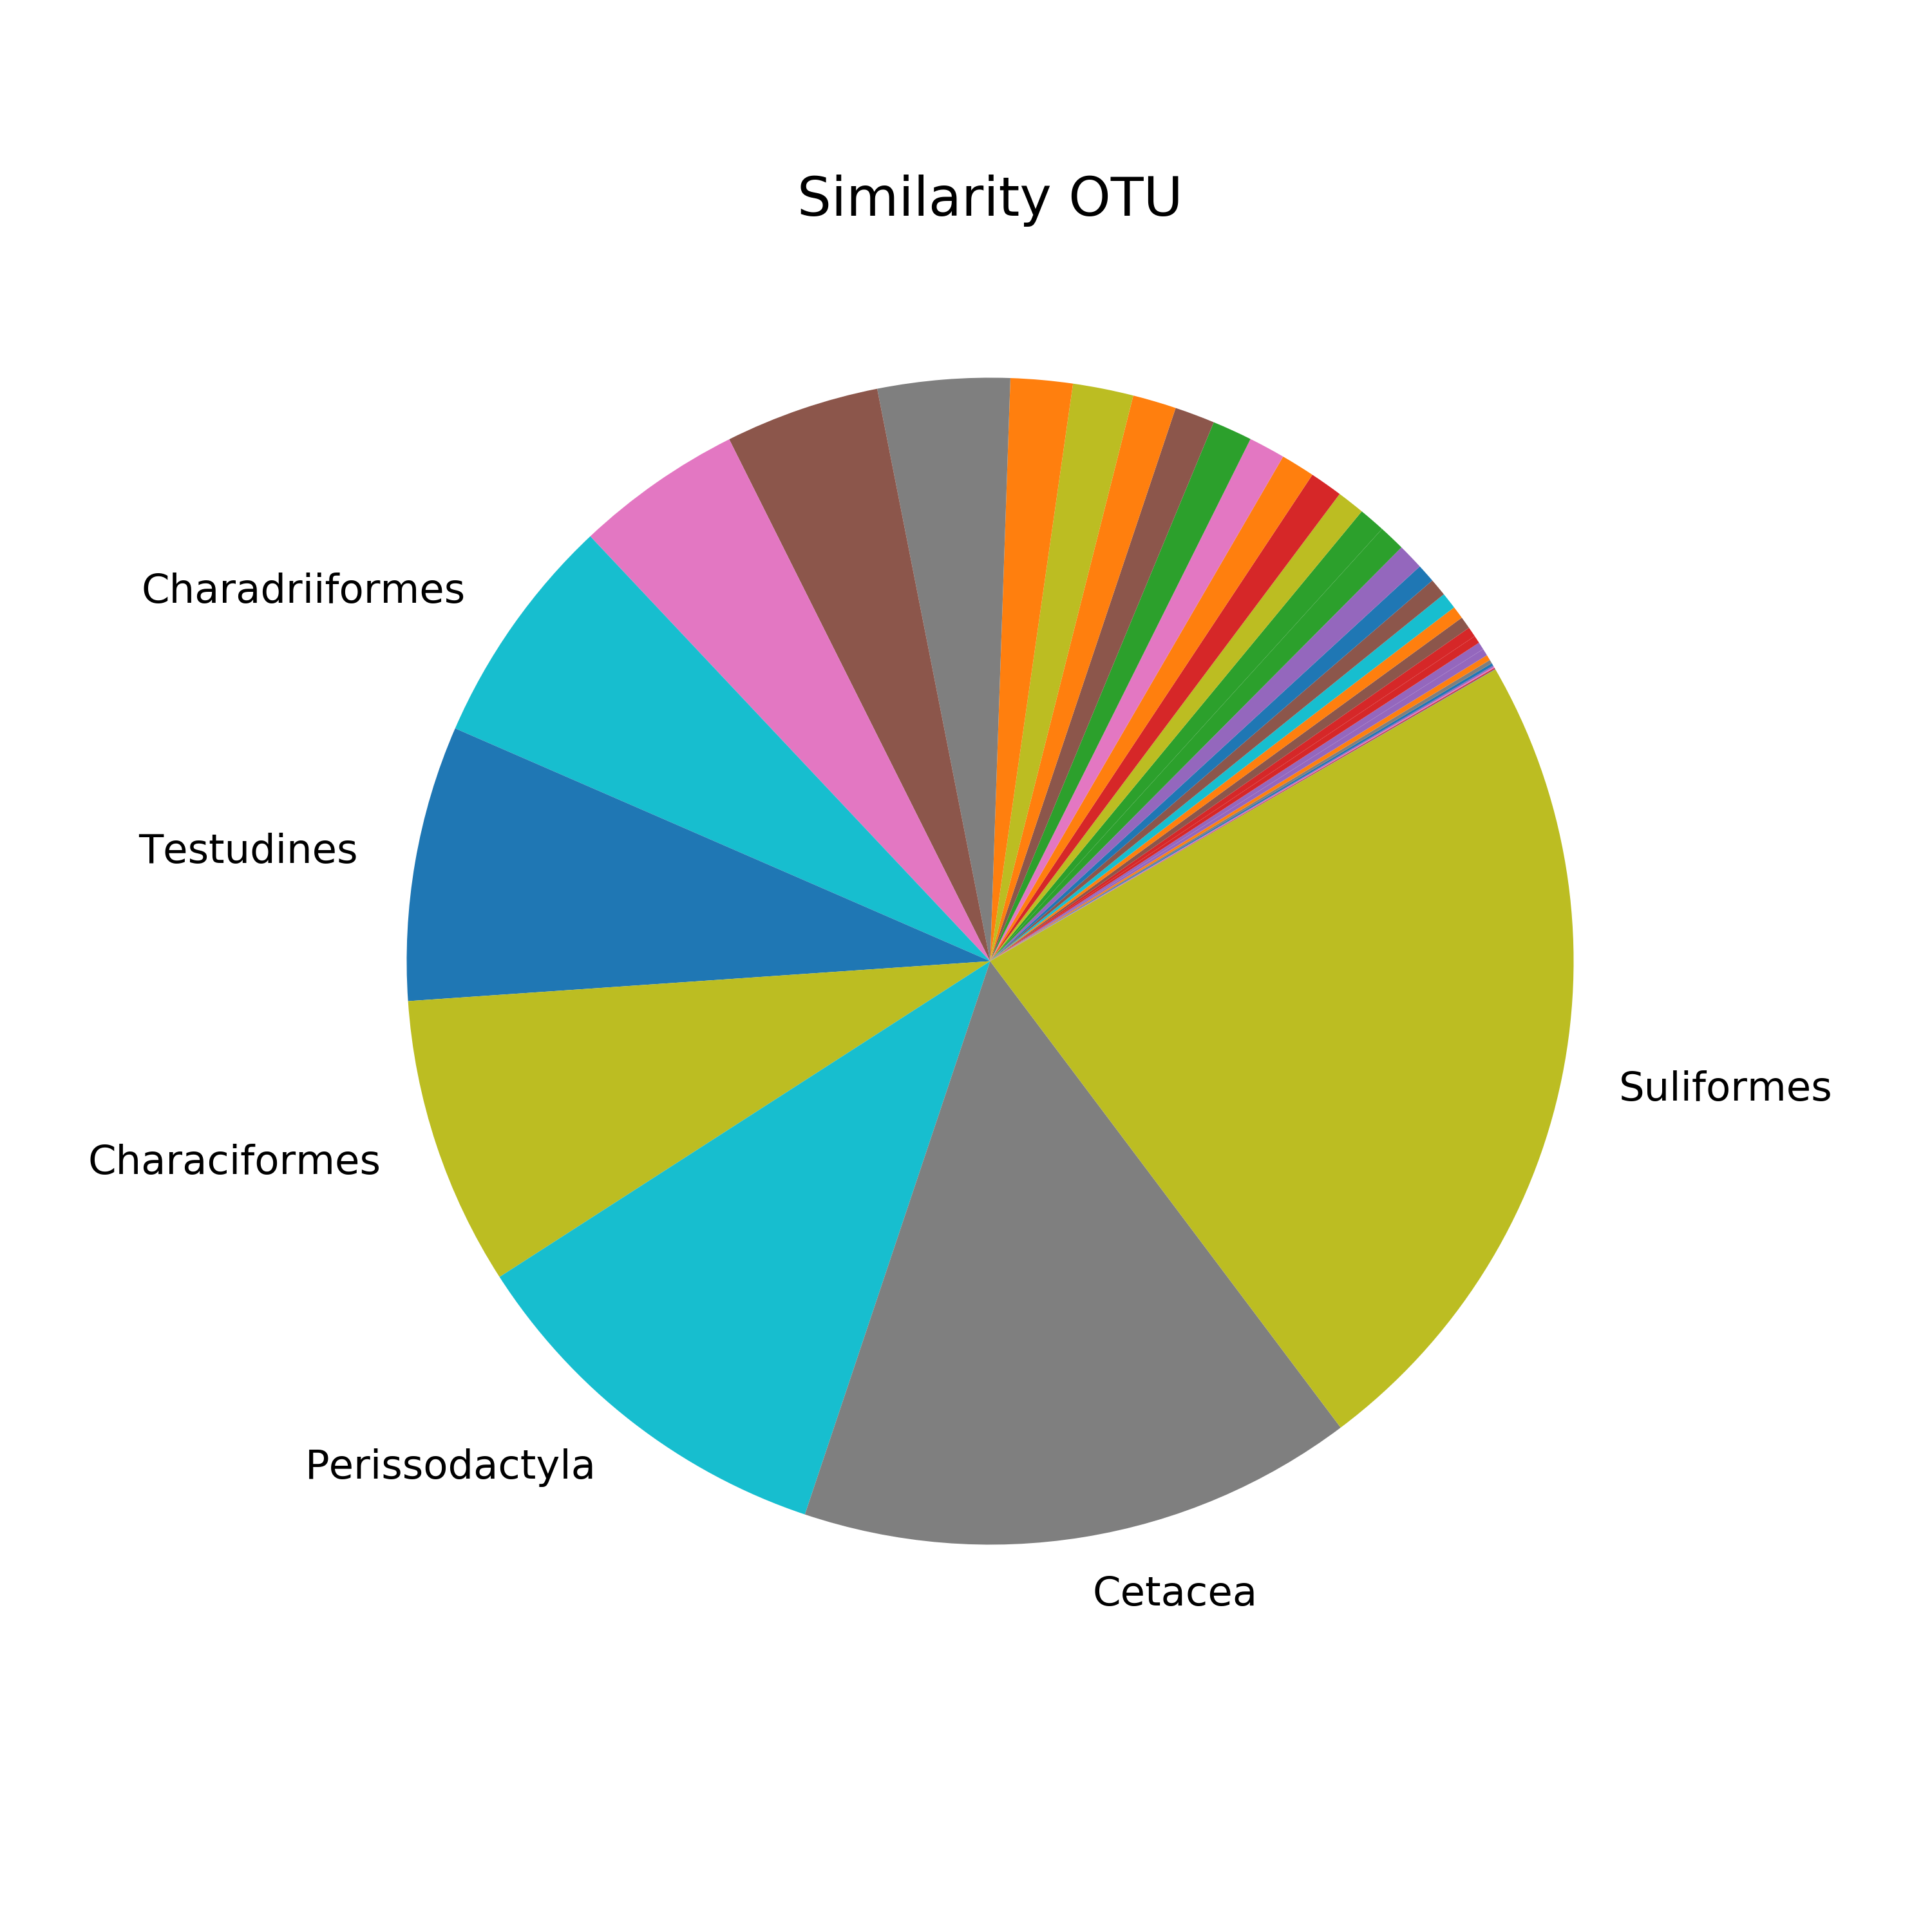
\includegraphics[width=\textwidth]{rfr_sim_order_pieOTU}
	\end{subfigure}
%		\begin{subfigure}{0.45\textwidth}
%		\includegraphics[width=\textwidth]{"rfr_sim_order_pieOTU\ CSS"}
%	\end{subfigure}\\
%	\begin{subfigure}{0.5\textwidth}
%		\includegraphics[width=\textwidth]{{rfr_sim_order_pieOTU\ MIN\ CSS}.png}
%	\end{subfigure}
\end{figure}